\documentclass[12pt]{article}
% include the pckage of the color%
\usepackage[usenames, dvipsnames]{color}
\usepackage[english]{babel}
\usepackage[utf8x]{inputenc}
\usepackage{amsmath}
\usepackage{graphicx}
\usepackage{subfiles}

%define your own color %
\definecolor{mygray}{gray}{0.9}
\begin{document}
	\listoffigures
	\title{Chapter 1 : General Project Presentation}
	\maketitle

	\section{Host Company Presentation}
	
	\subsection{Presentation of MASS Analytics}
	MASS Analytics, a Tunisian start-up founded in 2012, is the first and only independent Marketing Mix Modeling (MMM) agency in the MENA region. MASS Analytics’ core competency is the deep analysis and understanding of what impacts the consumer's path to purchase to make companies more effective with their marketing budget.
	\\
	\\
	It was founded by \textbf{Dr. Ramla Jarrar } ( Chief Executive Officer ),  \textbf{Dr. Firas Jabloun } (Chief Technology Officer), \textbf{Nadia Bouzguenda} (Business Development Director) \& \textbf{Rafal Kozlowski} (Director). They brought the essence of more than 20 cumulative years of experience in marketing effectiveness \& technology services at the international level to the creation of MASS-Analytics. [1]
	\\
	\\
	\begin{figure}[h]
	\centering
	
\includegraphics[width=0.2\textwidth]{Mass_logo.png}
	\caption{Mass-Analytics logo}
    \end{figure}
	\subsection{Services}
	\begin{itemize}
		\item \textbf{MassTer Software :} MASS Analytics has been developing internally its own Marketing Mix Modeling Software ``MassTer''. It is one of the most powerful Marketing Mix Modeling software products/solutions in the world and comes in three packages: standard, professional , and premium. It provides the user with a powerful Modeling platform coupled with a comprehensive data visualization capability to help understand the relationship between different variables and measure their impact on business performance.
			\begin{figure}[h]
			\centering
			
\includegraphics[width=0.3\textwidth]{massTer_logo.png}
			\caption{MassTer Software logo}
		\end{figure}
		
		\item \textbf{Training and Consultancy :} MASS Analytics runs specific courses and training sessions on advanced predictive modeling (log linear, nested modeling, fixed effect modeling…), budget optimization and return on Investment calculation. It alsooffers its clients coaching sessions to help improve their marketing analytics process and project delivery.
	\end{itemize}
\vspace{66mm}
	\subsection{Customers}
	
		\begin{figure}[h]
		\centering
		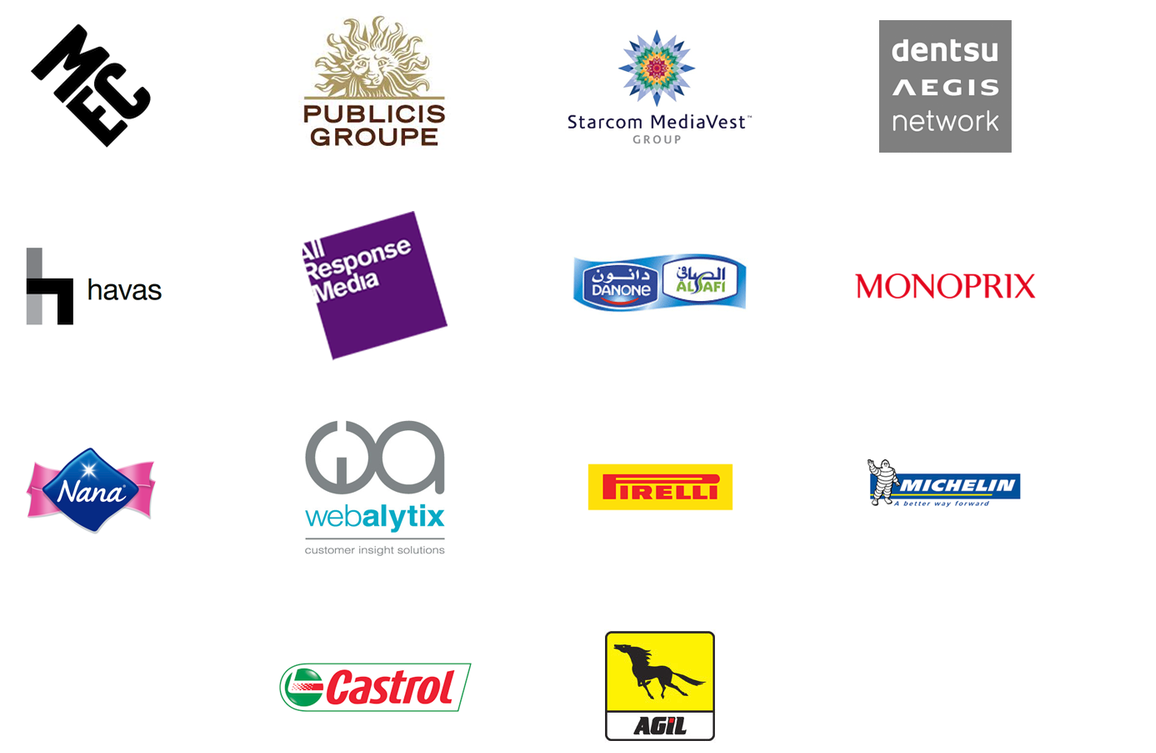
\includegraphics[width=0.8\textwidth]{customers_logo.png}
		\caption{Some of MASS Analytics’ customers logo}
	\end{figure}
	\section{Project Presentation}
	This part discusses the context of the project, presents the existent and the proposed solution as well as the objectives of the project.
	\subsection{General and Specific Objectives}
	The main objective of this project is to optimize the performance of the Auto-modeler module in terms of convergence and stability. In other respects, working on this project is an opportunity to boost one’s programming skills and aggrandize the grasp of previously-acquired and newly-learned technologies and algorithms, the genetic algorithm for instance.
	\subsection{Existing Presentation}
	MassTer Insight is .....
	\subsection{Problematic}
	subSection for the Problematic ....
	\subsection{Proposed Solution}
	subSection for the Proposed Solutions ....
	\subsection{Methodology}
	The choice of the methodology is an important step in software development since it grants formalizing the preliminary steps when establishing a system in pursuance of the client’s requirements.
	The  ? scrum ? TDD, an approach that is part of the Agile movement, was used when carrying out this project.
	\subsection{Conclusion}
	This chapter was a presentation of the hosting company, its services, and clients. The problematic of the project was also highlighted, along with the proposed solution and the methodology followed while carrying out the project.
	
\end{document}
